\documentclass{article}
\usepackage[utf8]{inputenc}
\usepackage{amsmath}
\usepackage{amssymb}
\usepackage{booktabs}
\usepackage{graphicx}
\usepackage{fancybox}
\usepackage{listings}
\usepackage{tikz}

% Definición de colores
\definecolor{azul}{RGB}{20, 100, 180}
\definecolor{verde}{RGB}{50, 150, 50}
\definecolor{naranja}{RGB}{255, 120, 0}

\title{ {Análisis de Componentes Multimedia en Aplicaciones Móviles}}
\author{Emmanuel Buenrostro Briseño}
\date{\today}

\begin{document}
\maketitle

\section{Introducción}
Los componentes multimedia y de hardware son esenciales para construir aplicaciones móviles con más funcionalidades. Su integración va más allá de lo visual, potenciando la funcionalidad y la experiencia del usuario. 

\hrule

\section{Componentes Multimedia y de Hardware}

La siguiente tabla resume los principales componentes, su función y uso más común:
\newpage
\begin{table}[h]
    \centering
    
    \begin{tabular}{|p{2.5cm}|p{5cm}|p{6cm}|}
        \toprule
         {Componente} &  {Función Principal} &  {Uso Frecuente en Apps} \\
        \midrule
         {Imágenes} & Definir la Interfaz de Usuario , mostrar contenido estático (iconos, fotos, gráficos). & Todas (E-commerce, Redes Sociales, Utilidades). \\
        \midrule
         {Audio} & Proporcionar \textit{feedback} sonoro, música de fondo, notificaciones y contenido de voz. & Reproductores de \textit{Podcast}/Música (Spotify), Comunicación (\textit{VoIP}), Juegos. \\
        \midrule
         {Video} & Transmisión de contenido (\textit{streaming}), tutoriales, publicidad y captura/reproducción por el usuario. & Plataformas de \textit{Streaming} (Netflix), Redes Sociales de video (TikTok), Editores. \\
        \midrule
         {Animaciones} & Facilitar transiciones, indicar estados de carga, mejorar la fluidez y dar \textit{feedback} visual. &  {Todas} (UI/UX), Juegos, \textit{Onboarding} de usuarios. \\
        \midrule
         {Cámara} & Capturar fotos/videos, escanear códigos (QR/documentos) e implementar  {Realidad Aumentada (RA)}. & Redes Sociales, \textit{Scanners} de Documentos, \textit{Apps} de Fotografía/Edición, RA (filtros). \\
        \midrule
         {Sensores} & Recolectar datos del entorno y movimiento ( {Acelerómetro, GPS, Giroscopio}) para interacción posicional. & Navegación (Waze), \textit{Fitness}/\textit{Trackers} de salud (Strava), Juegos de RA (Pokémon GO). \\
        \bottomrule
    \end{tabular}
\end{table}

\hrule

\section{Evidencias del Análisis}

\subsection{Diagrama Esquemático}

El siguiente diagrama representa la interacción funcional de los componentes multimedia y de \textit{hardware} en una aplicación de captura de contenido (ejemplo: una red social de video).


\begin{center}
    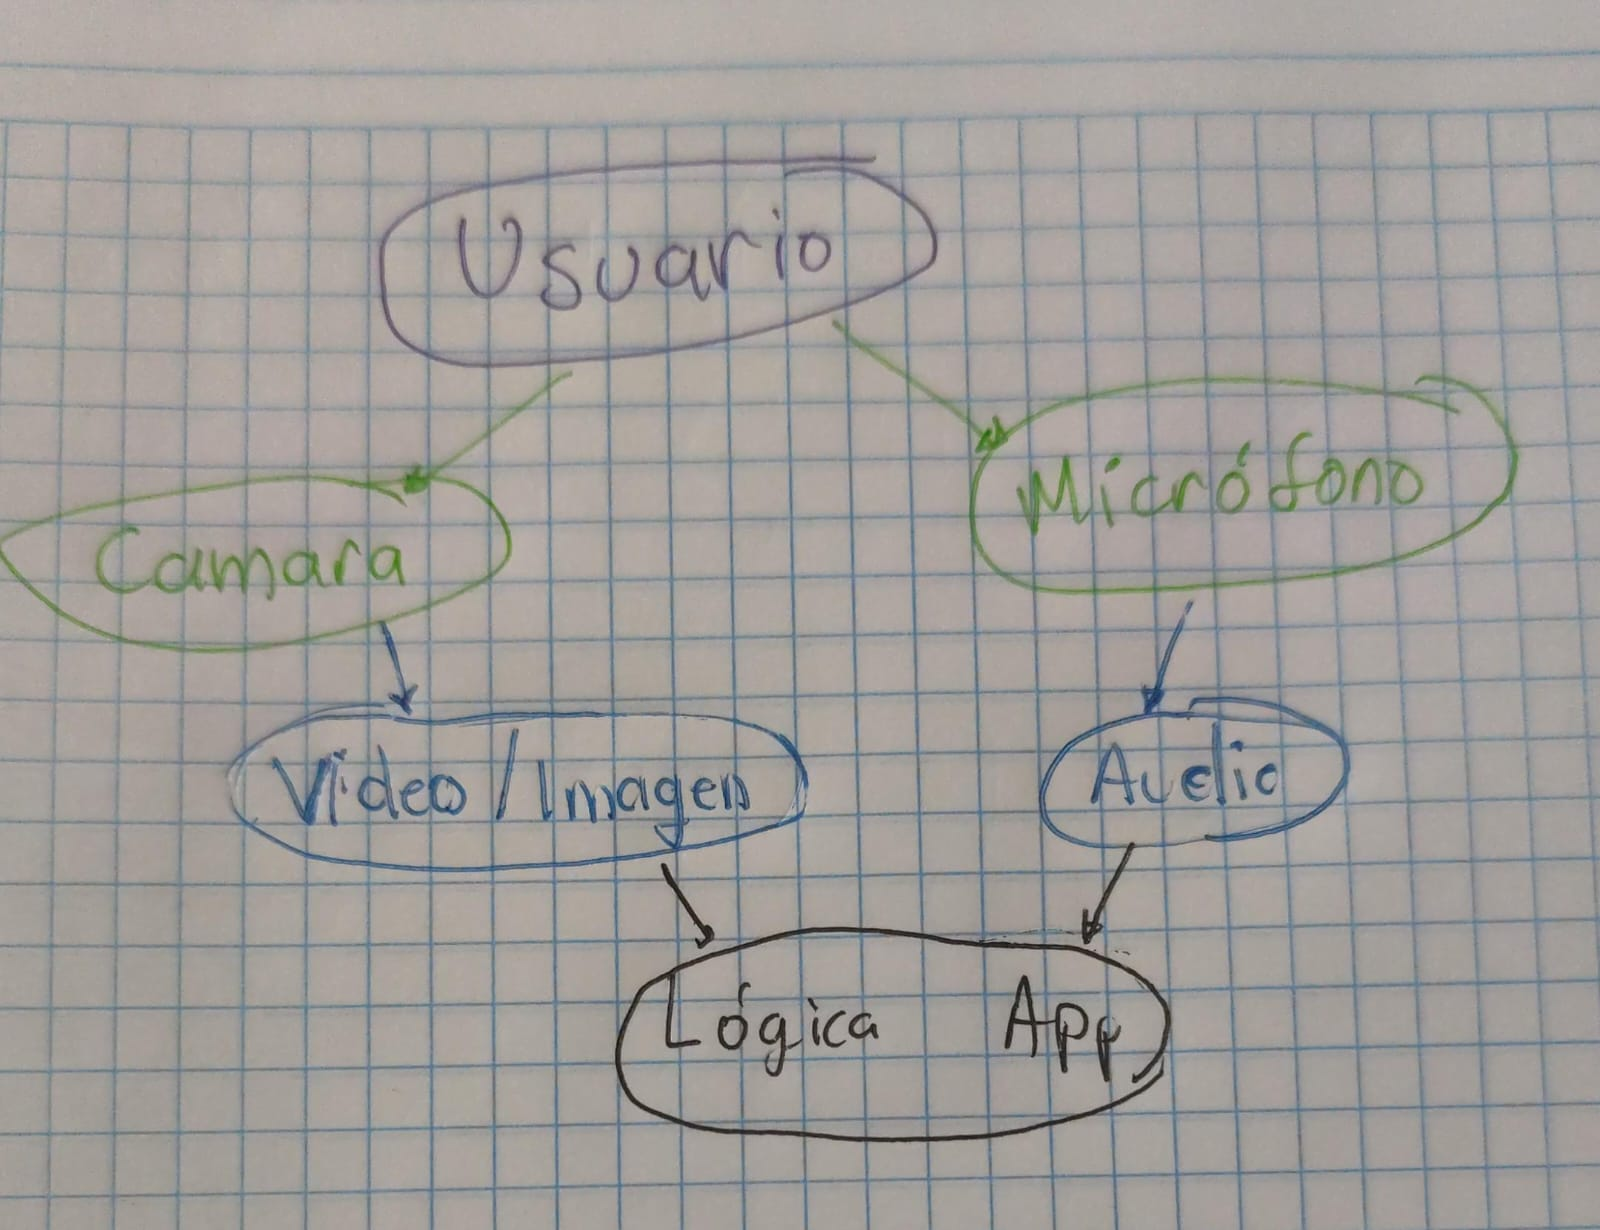
\includegraphics[scale=0.2]{diagrama.jpg}
\end{center}


\subsection{Notas y Comentarios Personales}


\subsection{Ejemplos de Aplicaciones y su Integración}

\begin{itemize}
    \item  {Aplicación:}  {Spotify/Netflix}.
    \begin{itemize}
        \item  {Componente Clave:}  {Audio} y  {Video} (streaming optimizado).
        \item  {Función:} Reproducción de contenido. Utilizan animaciones sutiles en la UI para indicar el progreso de la reproducción y transiciones.
    \end{itemize}

    \item  {Aplicación:}  {Waze/Google Maps}.
    \begin{itemize}
        \item  {Componente Clave:}  {Sensores (GPS)}.
        \item  {Función:} Navegación y geolocalización. El componente de  {Audio} se usa para dar indicaciones de voz, minimizando la necesidad de interacción visual.
    \end{itemize}

\end{itemize}

\end{document}